\documentclass[11pt,a4paper]{article}
\usepackage[utf8]{inputenc}
\usepackage{babel}
\usepackage{graphicx}
\usepackage{geometry}
\usepackage{float}
\usepackage{hyperref}
\usepackage{booktabs}
\usepackage{amsmath}
\usepackage{array}
\usepackage{xcolor}
\geometry{margin=2.5cm}

% Rutas para figuras tanto si se compila desde raíz como desde parcial2/
\graphicspath{{./}{parcial2/}}

% ─── Colores institucionales ───────────────────────────────────────────────────
\definecolor{verde}{RGB}{26,77,46}
\definecolor{naranja}{RGB}{232,110,56}

\begin{document}

% =============================================================================
% PORTADA
% =============================================================================
\begin{titlepage}
    \centering
    \vspace*{1.5cm}

    {\Huge \textbf{Universidad Tecnológica de la Mixteca}}\\[1.5cm]

    {\huge \textbf{Procesamiento de Imágenes de Plantas \\
    para la Detección de Plagas}}\\[1.2cm]

    {\Large \textcolor{verde}{\textbf{Segundo Parcial: Segmentación de Imágenes}}}\\[0.8cm]

    {\large Procesamiento Digital de Imágenes}\\[2.0cm]

    {\large \textbf{Alumno:}}\\
    {\Large Irving Tristán Pérez Zurita}\\[0.5cm]

    {\large \textbf{Grupo:}}\\
    {\Large 902-A}\\[1.5cm]

    {\large \textbf{Profesora:}}\\
    {\Large Dra.\ Verónica Rodríguez López}\\[1.5cm]

    \vfill
    {\large \today}
\end{titlepage}

\newpage
\tableofcontents
\newpage

% =============================================================================
\section{Clasificación de las imágenes por nivel de complejidad}
% =============================================================================

Las imágenes del \textit{New Plant Diseases Dataset} presentan características
visuales muy distintas que determinan qué tan difícil es aislar la hoja del
fondo. Se identificaron tres niveles de complejidad con base en criterios
morfológicos, fotométricos y de fondo:

\begin{table}[H]
    \centering
    \renewcommand{\arraystretch}{1.4}
    \begin{tabular}{@{} >{\bfseries}p{2.8cm} p{3.8cm} p{3.8cm} p{3.8cm} @{}}
        \toprule
        Criterio
            & \textcolor{verde}{\textbf{Complejidad Baja}}
            & \textcolor{naranja}{\textbf{Complejidad Media}}
            & \textbf{Complejidad Alta} \\
        \midrule
        Fondo
            & Homogéneo, liso y neutro (blanco/gris de laboratorio)
            & Superficie lisa con sombras arrojadas
            & Textura compleja, tallos u hojas de fondo \\
        Iluminación
            & Uniforme y difusa, sin sombras duras
            & Gradientes de luz y brillos especulares
            & Variación severa o baja relación contraste/ruido \\
        Estado de la hoja
            & Bordes lisos, tejido sano o síntomas leves
            & Lesiones necróticas, clorosis marrón/amarilla
            & Múltiples hojas solapadas o daño foliar extenso \\
        Histograma
            & Fuertemente bimodal con valle nítido
            & Bimodal degradado o multimodal
            & Modos solapados sin separación evidente \\
        Reto principal
            & Mínimo; umbralización directa funciona
            & Evitar confundir manchas y sombras con el fondo
            & Agrupamiento multidimensional y filtrado estricto \\
        \bottomrule
    \end{tabular}
    \caption{Criterios de clasificación por nivel de complejidad visual.}
    \label{tab:complejidad}
\end{table}

% =============================================================================
\section{Diagramas de flujo de preprocesamiento y segmentación}
% =============================================================================

Para cada nivel de complejidad se diseñó un flujo de procesamiento específico,
ajustando el algoritmo de segmentación y sus parámetros a las condiciones
visuales de la imagen.

% ─────────────────────────────────────────────────────────────────────────────
\subsection{Caso 1 — Complejidad Baja: Umbralización global y Otsu}
% ─────────────────────────────────────────────────────────────────────────────

Las imágenes de complejidad baja poseen un histograma marcadamente bimodal,
lo que permite segmentar la hoja con un único umbral calculado de forma
automática u óptima.

\begin{figure}[H]
    \centering
    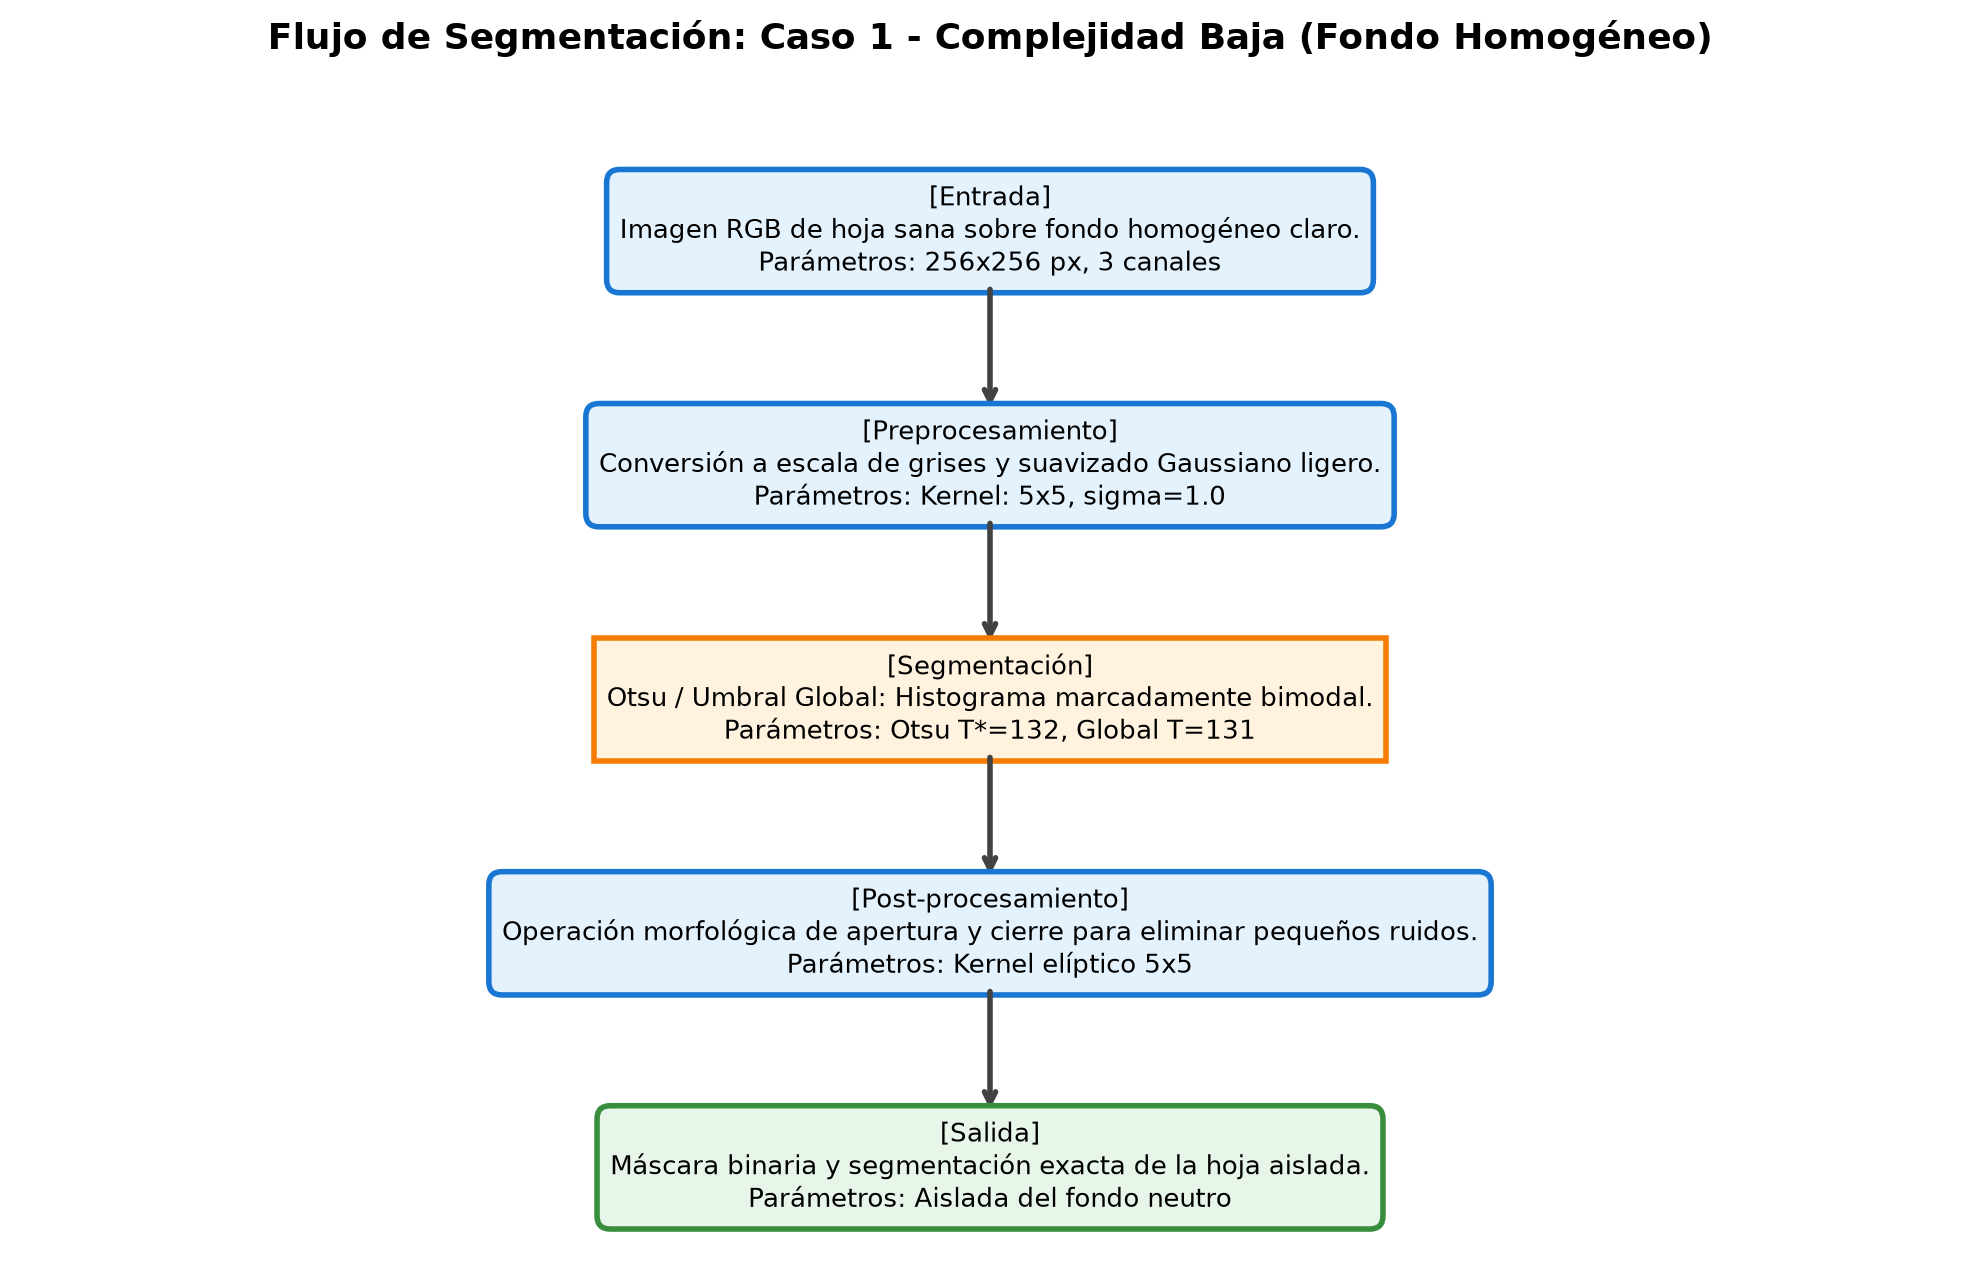
\includegraphics[width=0.80\textwidth]{resultados/diagramas/flujo_baja_complejidad.png}
    \caption{Diagrama de flujo para imágenes de complejidad baja. El histograma
    bimodal permite aplicar directamente Umbralización Global o Otsu con alta
    precisión.}
    \label{fig:flujo_baja}
\end{figure}

\begin{table}[H]
    \centering
    \renewcommand{\arraystretch}{1.3}
    \begin{tabular}{@{}lll@{}}
        \toprule
        \textbf{Etapa} & \textbf{Parámetro} & \textbf{Valor} \\ \midrule
        Suavizado Gaussiano & Kernel / $\sigma$ & $5\times5$ / 1.0 \\
        Umbral Global (G\&W) & $\delta T$ / Max. iteraciones & 0.5 / 100 \\
        Umbral de Otsu & Espacio / Inversión & Canal $a^*$ LAB / THRESH\_BINARY\_INV \\
        Morfología post. & Kernel & Elipse $5\times5$ (apertura + cierre) \\
        \bottomrule
    \end{tabular}
    \caption{Parámetros del flujo para complejidad baja.}
    \label{tab:params_baja}
\end{table}

% ─────────────────────────────────────────────────────────────────────────────
\subsection{Caso 2 — Complejidad Media: K-Means y Canny}
% ─────────────────────────────────────────────────────────────────────────────

Las sombras y manchas de enfermedades confunden los métodos de umbralización
simple. K-Means en espacio L*a*b* con $K=3$ permite separar fondo, tejido
sano y áreas enfermas; Canny con ajuste de histéresis detecta los contornos
continuos de la hoja.

\begin{figure}[H]
    \centering
    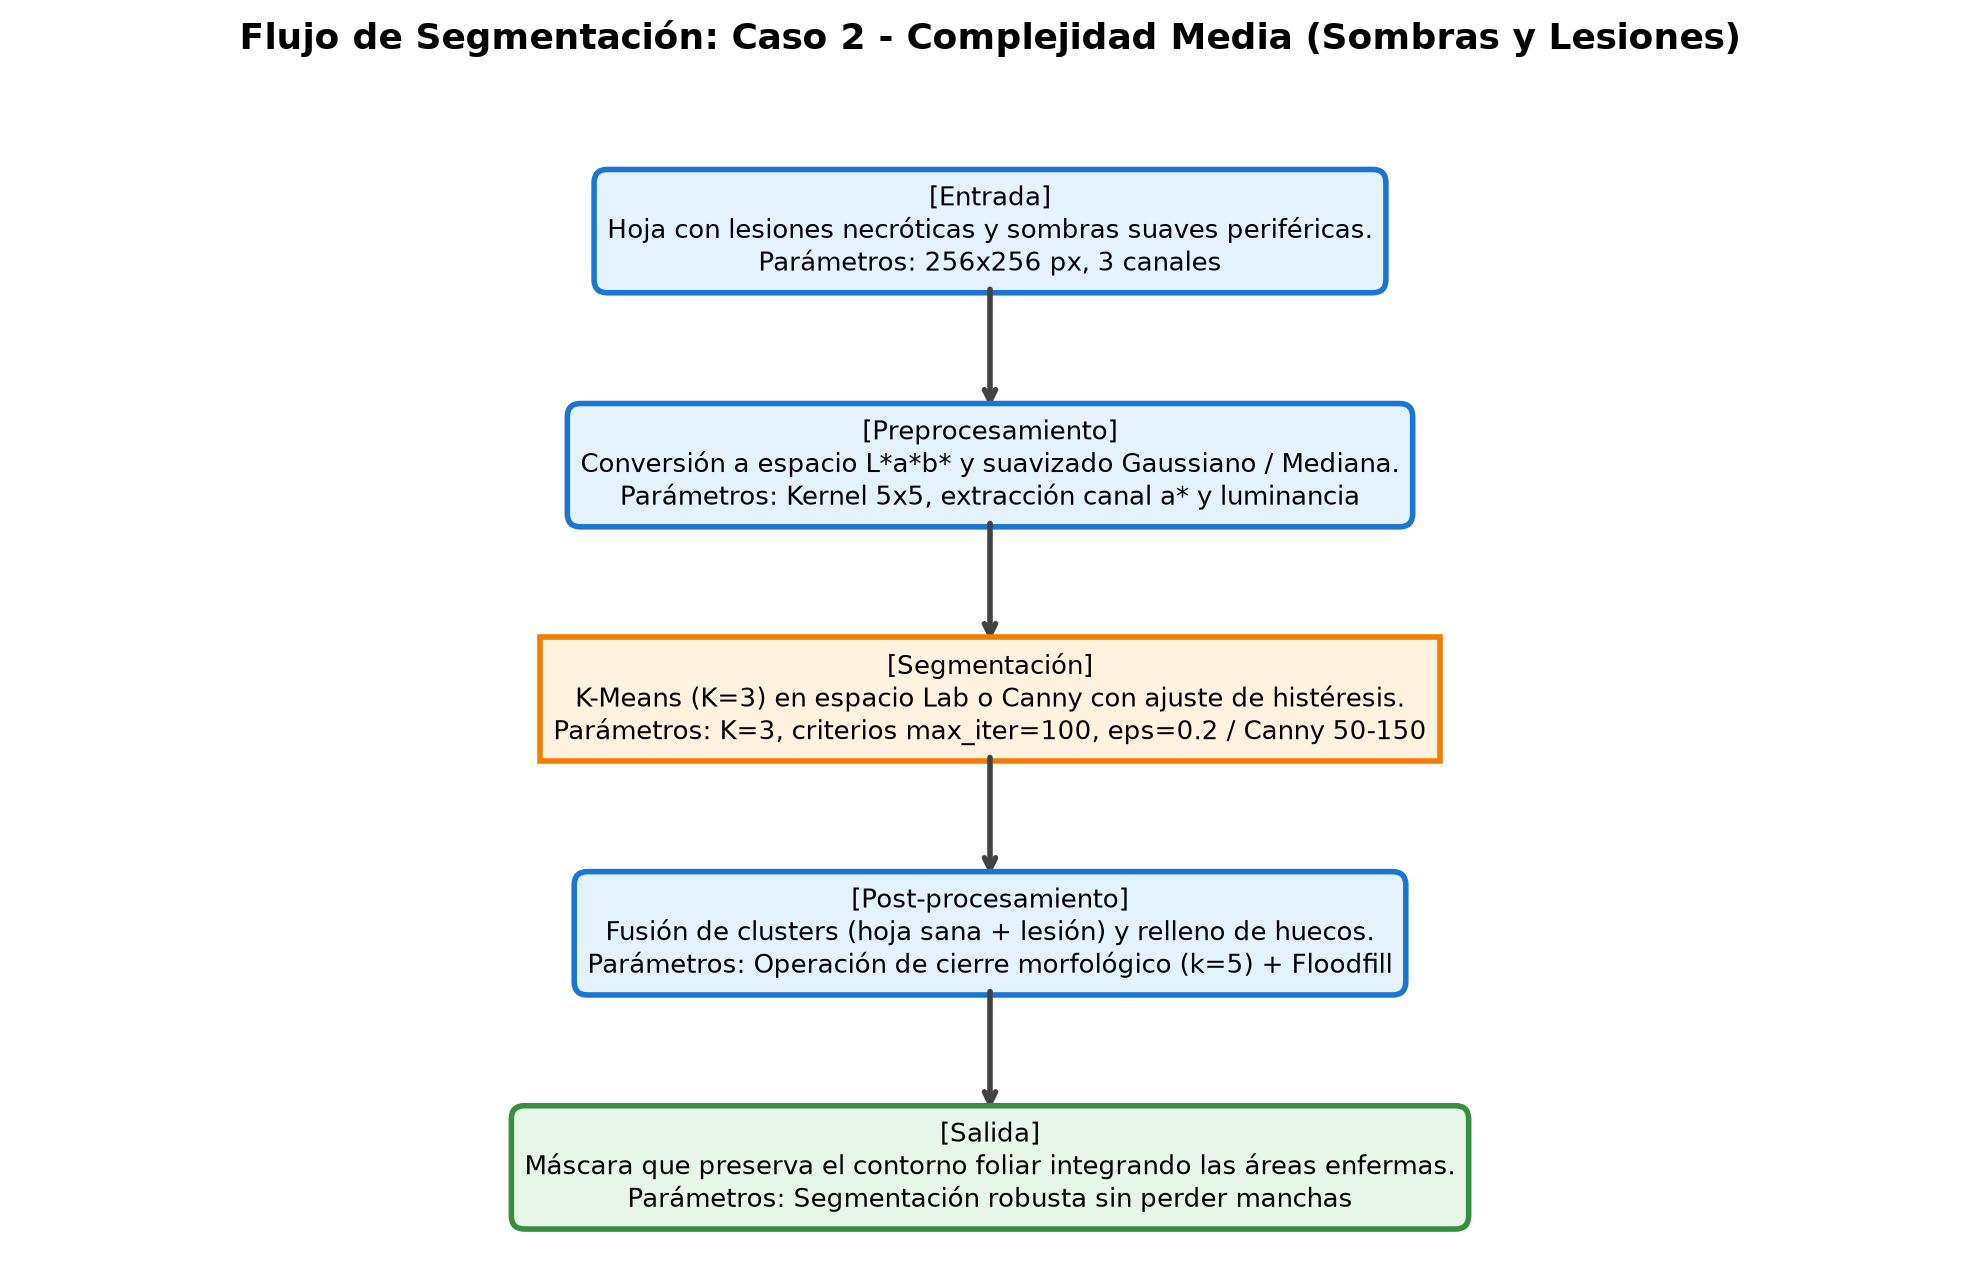
\includegraphics[width=0.80\textwidth]{resultados/diagramas/flujo_media_complejidad.png}
    \caption{Diagrama de flujo para imágenes de complejidad media. Se combina
    la información del canal $a^*$ (sensible al verde) con la segmentación por
    clusters para incluir las áreas patológicas.}
    \label{fig:flujo_media}
\end{figure}

\begin{table}[H]
    \centering
    \renewcommand{\arraystretch}{1.3}
    \begin{tabular}{@{}lll@{}}
        \toprule
        \textbf{Etapa} & \textbf{Parámetro} & \textbf{Valor} \\ \midrule
        Preprocesamiento & Suavizado Gaussiano & $5\times5$, $\sigma=1.0$ \\
        Canny & $T_{\text{low}}$ / $T_{\text{high}}$ & 50 / 150 \\
        Canny — Morfología & Kernel cierre & Elipse $5\times5$, 2 iteraciones \\
        K-Means & $K$ / Espacio color & 3 / L*a*b* \\
        K-Means — Criterio & Max. iter.\ / $\varepsilon$ & 100 / 0.2 \\
        K-Means — Post. & Kernel morfológico & Elipse $5\times5$ (apertura + cierre) \\
        \bottomrule
    \end{tabular}
    \caption{Parámetros del flujo para complejidad media.}
    \label{tab:params_media}
\end{table}

% ─────────────────────────────────────────────────────────────────────────────
\subsection{Caso 3 — Complejidad Alta: K-Means multicanal y Canny ajustado}
% ─────────────────────────────────────────────────────────────────────────────

Las imágenes con fondo complejo requieren un preprocesamiento más robusto
(Filtro Bilateral para preservar bordes), umbrales Canny más bajos para
capturar detalles finos, y post-procesamiento con convex hull para descartar
artefactos del fondo.

\begin{figure}[H]
    \centering
    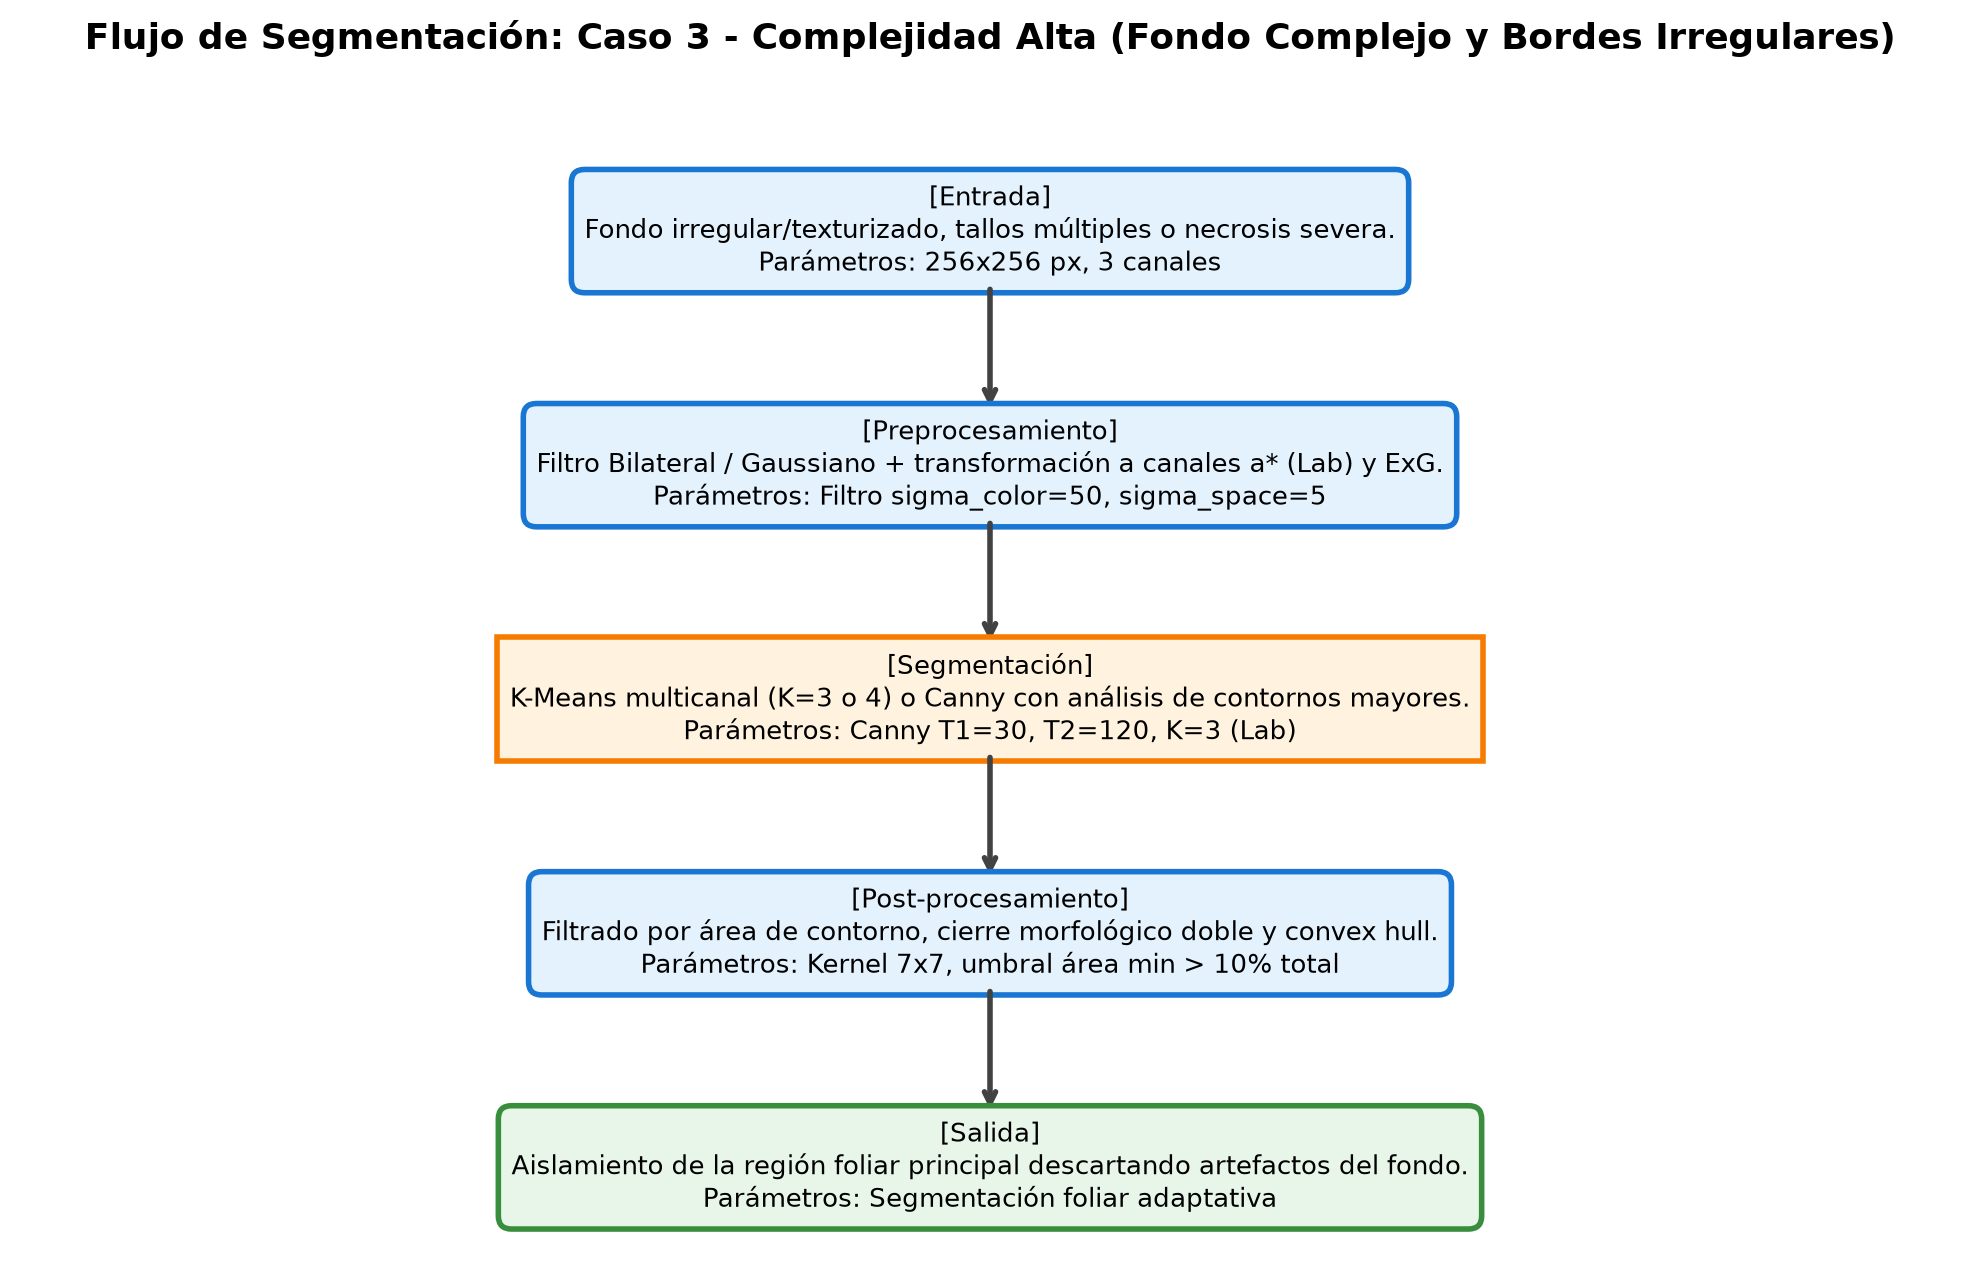
\includegraphics[width=0.80\textwidth]{resultados/diagramas/flujo_alta_complejidad.png}
    \caption{Diagrama de flujo para imágenes de complejidad alta. Se emplea
    el Filtro Bilateral como preprocesamiento y umbrales Canny adaptados al
    menor contraste disponible.}
    \label{fig:flujo_alta}
\end{figure}

\begin{table}[H]
    \centering
    \renewcommand{\arraystretch}{1.3}
    \begin{tabular}{@{}lll@{}}
        \toprule
        \textbf{Etapa} & \textbf{Parámetro} & \textbf{Valor} \\ \midrule
        Preprocesamiento & Filtro Bilateral ($d$/$\sigma_c$/$\sigma_s$) & 5 / 50 / 50 \\
        Canny & $T_{\text{low}}$ / $T_{\text{high}}$ & 30 / 120 \\
        Canny — Morfología & Kernel cierre & Elipse $7\times7$, 2 iteraciones \\
        K-Means & $K$ / Espacio color & 3 / L*a*b* \\
        Post-proceso & Umbral área mínima & $>$ 10\% del área total \\
        Post-proceso & Kernel morfológico & Elipse $7\times7$ (cierre doble) \\
        \bottomrule
    \end{tabular}
    \caption{Parámetros del flujo para complejidad alta.}
    \label{tab:params_alta}
\end{table}

% =============================================================================
\section{Fundamento teórico de los algoritmos implementados}
% =============================================================================

\subsection{Detector de bordes de Canny (1986)}

Opera en cuatro etapas secuenciales:

\begin{enumerate}
    \item \textbf{Suavizado Gaussiano:} reduce el ruido de alta frecuencia antes
    de calcular derivadas, usando $G(x,y) = \exp\!\bigl(-(x^2+y^2)/(2\sigma^2)\bigr)$.

    \item \textbf{Gradiente con operadores de Sobel:} calcula la magnitud
    $|\nabla f| = \sqrt{G_x^2 + G_y^2}$ y la dirección $\theta = \arctan(G_y/G_x)$.

    \item \textbf{Supresión de no máximos:} adelgaza los bordes a 1 píxel
    conservando únicamente los máximos locales en la dirección del gradiente.

    \item \textbf{Umbralización con histéresis:} utiliza dos umbrales $T_{\text{low}}$
    y $T_{\text{high}}$. Los píxeles con respuesta $> T_{\text{high}}$ son bordes
    seguros; los que superan $T_{\text{low}}$ se retienen solo si están conectados
    (8-conectividad) a un borde seguro.
\end{enumerate}

\subsection{Umbralización Global Iterativa (Gonzalez \& Woods)}

\[
T^{(n+1)} = \frac{\mu_1(T^{(n)}) + \mu_2(T^{(n)})}{2}
\]

donde $\mu_1$ y $\mu_2$ son las medias de los píxeles que superan y no
superan el umbral actual $T^{(n)}$, respectivamente. El proceso converge
cuando $|T^{(n+1)} - T^{(n)}| < \delta T$.

\subsection{Umbralización de Otsu (1979)}

Maximiza la varianza inter-clase:
\[
\sigma_B^2(t) = \omega_0(t)\,\omega_1(t)\,[\mu_0(t) - \mu_1(t)]^2
\]

El umbral óptimo $T^*$ se determina automáticamente sin intervención manual,
equivaliendo a minimizar la dispersión intra-clase.

\subsection{Agrupamiento K-Means}

Particiona los $N$ píxeles en $K$ clusters minimizando:
\[
J = \sum_{k=1}^{K} \sum_{\mathbf{x}_i \in C_k} \|\mathbf{x}_i - \boldsymbol{\mu}_k\|^2
\]

Se aplica en espacio de color L*a*b* para mejor separación perceptual entre
el fondo, el tejido vegetal sano y las lesiones patológicas.

% =============================================================================
\section{Resultados obtenidos}
% =============================================================================

Se procesaron tres imágenes representativas (una por nivel de complejidad)
aplicando los cuatro métodos de segmentación. Los resultados se muestran a
continuación.

% ─────────────────────────────────────────────────────────────────────────────
\subsection{Comparativa global por método y complejidad}
% ─────────────────────────────────────────────────────────────────────────────

\begin{figure}[H]
    \centering
    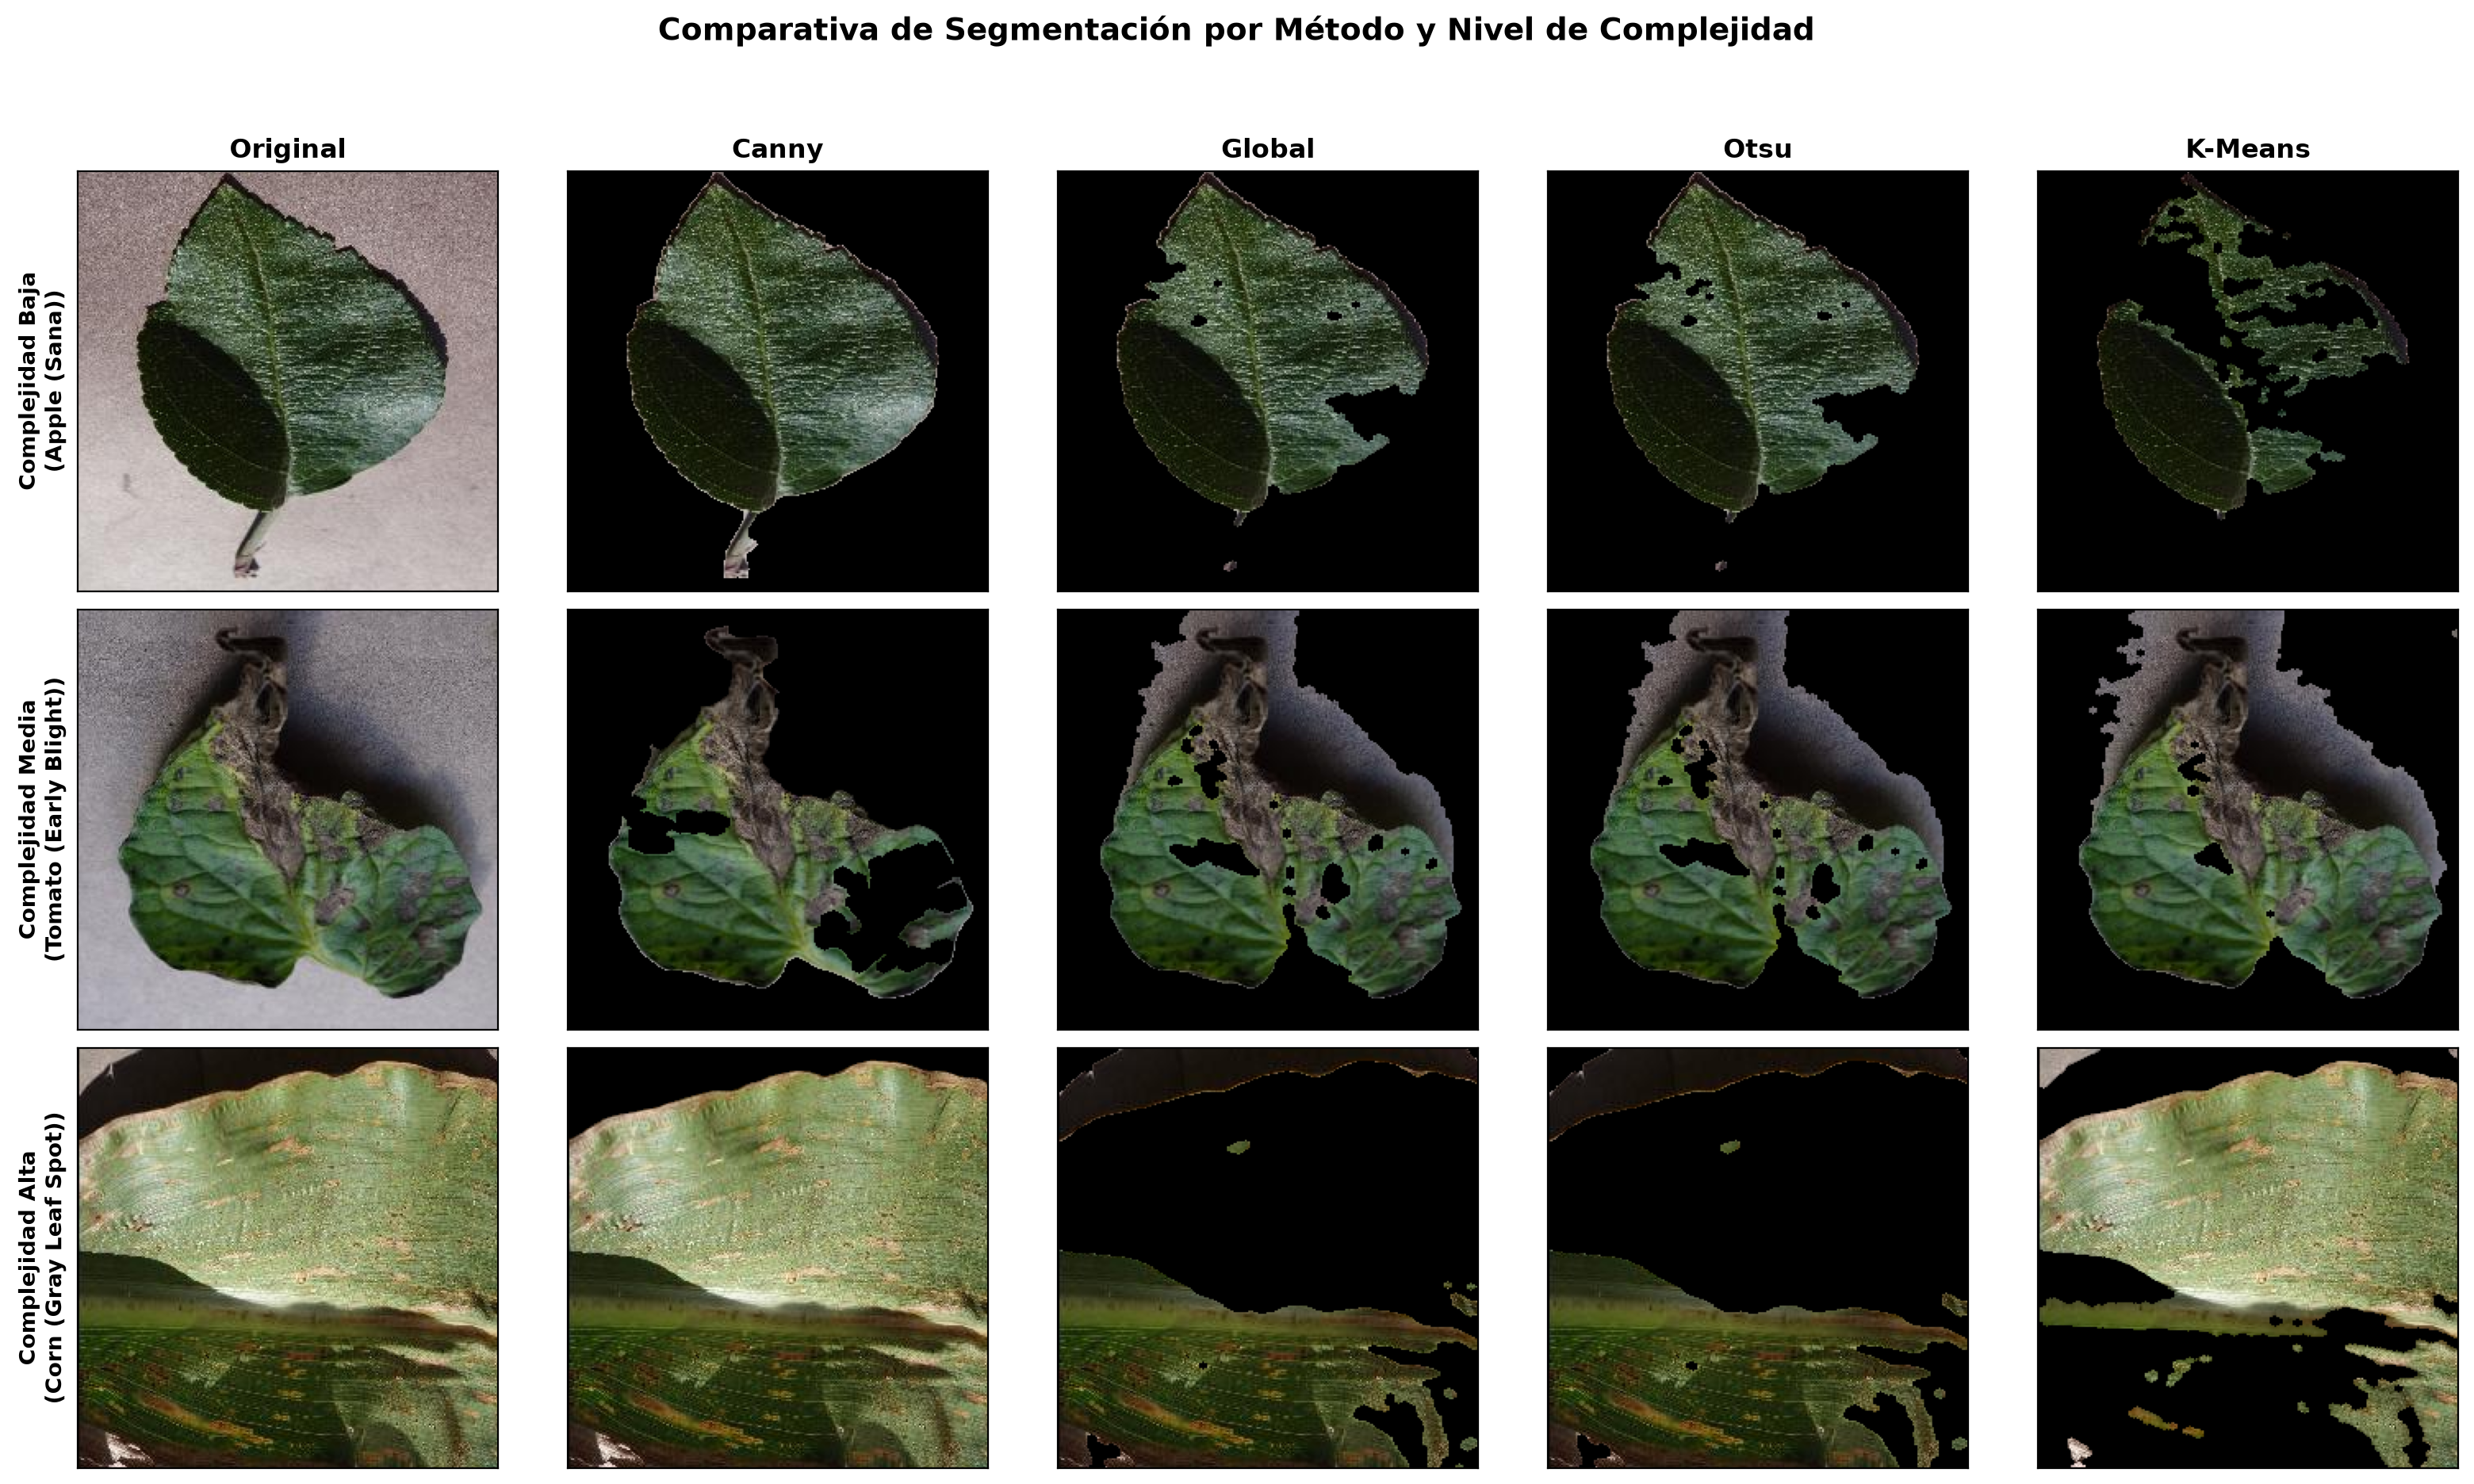
\includegraphics[width=\textwidth]{resultados/comparaciones/comparativa_global.png}
    \caption{Comparativa de los cuatro métodos de segmentación para los tres
    niveles de complejidad. Las columnas muestran (de izquierda a derecha):
    imagen original, Canny, Umbral Global, Otsu y K-Means.}
    \label{fig:comparativa_global}
\end{figure}

% ─────────────────────────────────────────────────────────────────────────────
\subsection{Caso 1 — Complejidad Baja}
% ─────────────────────────────────────────────────────────────────────────────

\begin{figure}[H]
    \centering
    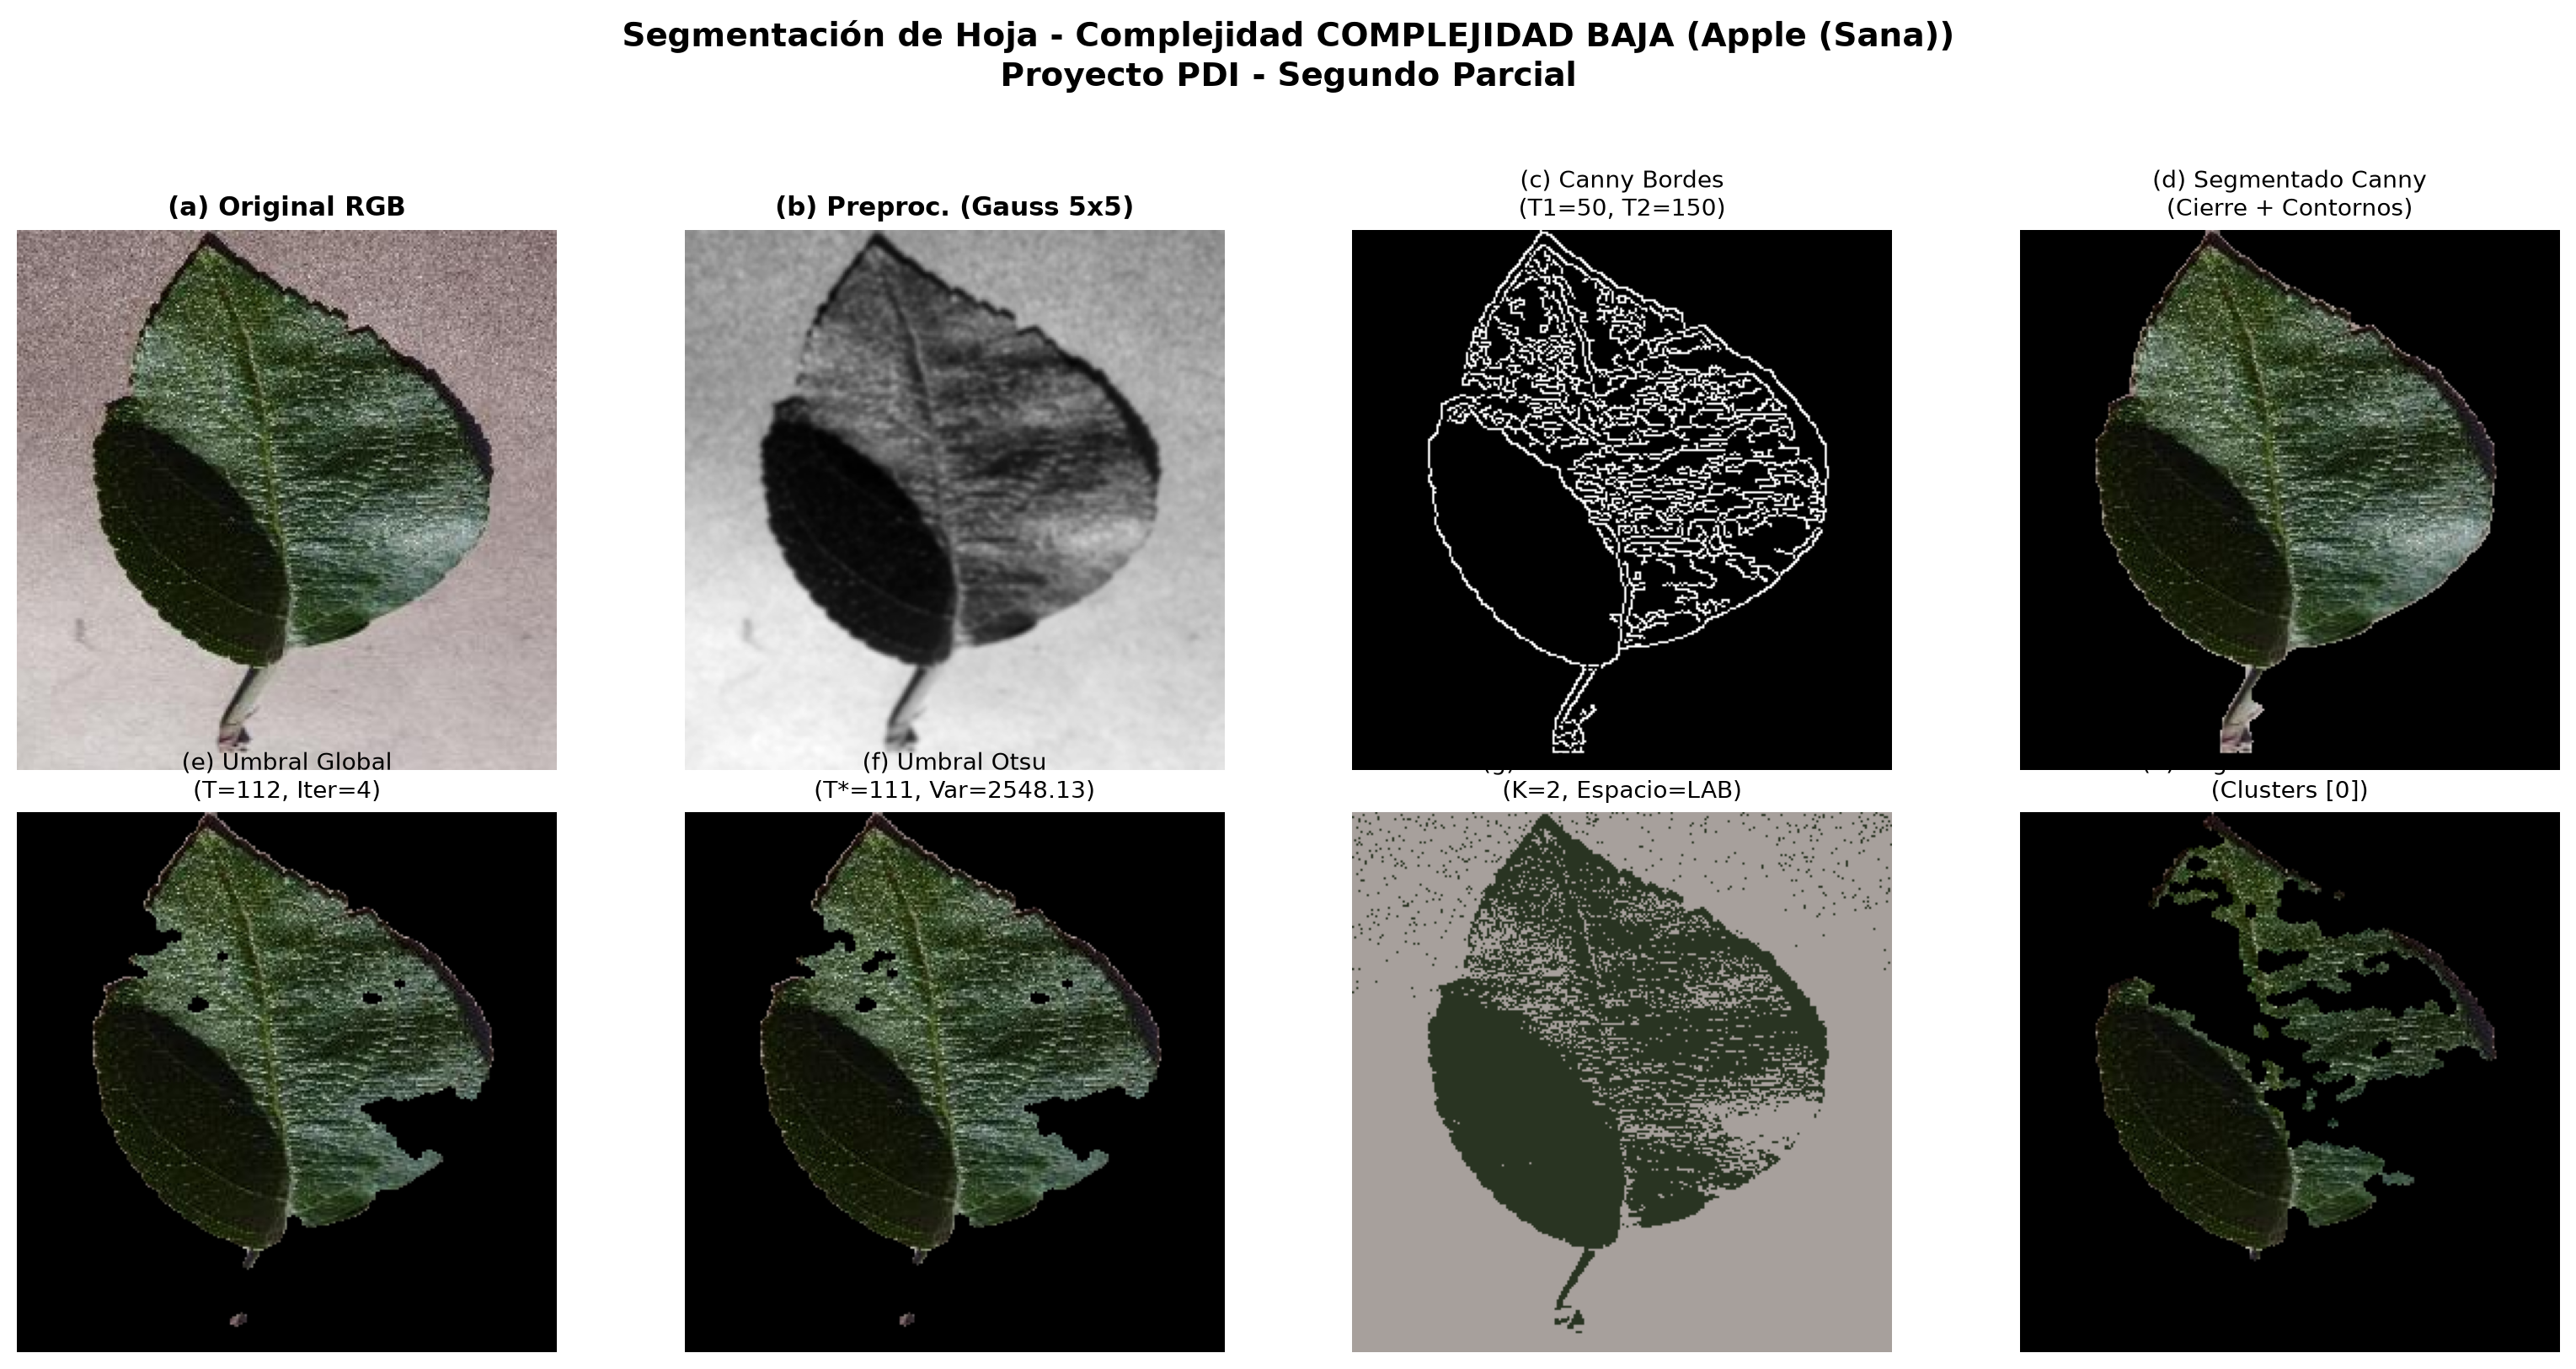
\includegraphics[width=\textwidth]{resultados/comparaciones/caso_baja.png}
    \caption{Resultados de segmentación para imagen de complejidad baja. El
    histograma bimodal permite a Otsu y al Umbral Global obtener una máscara
    casi perfecta sin post-procesamiento adicional.}
    \label{fig:caso_baja}
\end{figure}

% ─────────────────────────────────────────────────────────────────────────────
\subsection{Caso 2 — Complejidad Media}
% ─────────────────────────────────────────────────────────────────────────────

\begin{figure}[H]
    \centering
    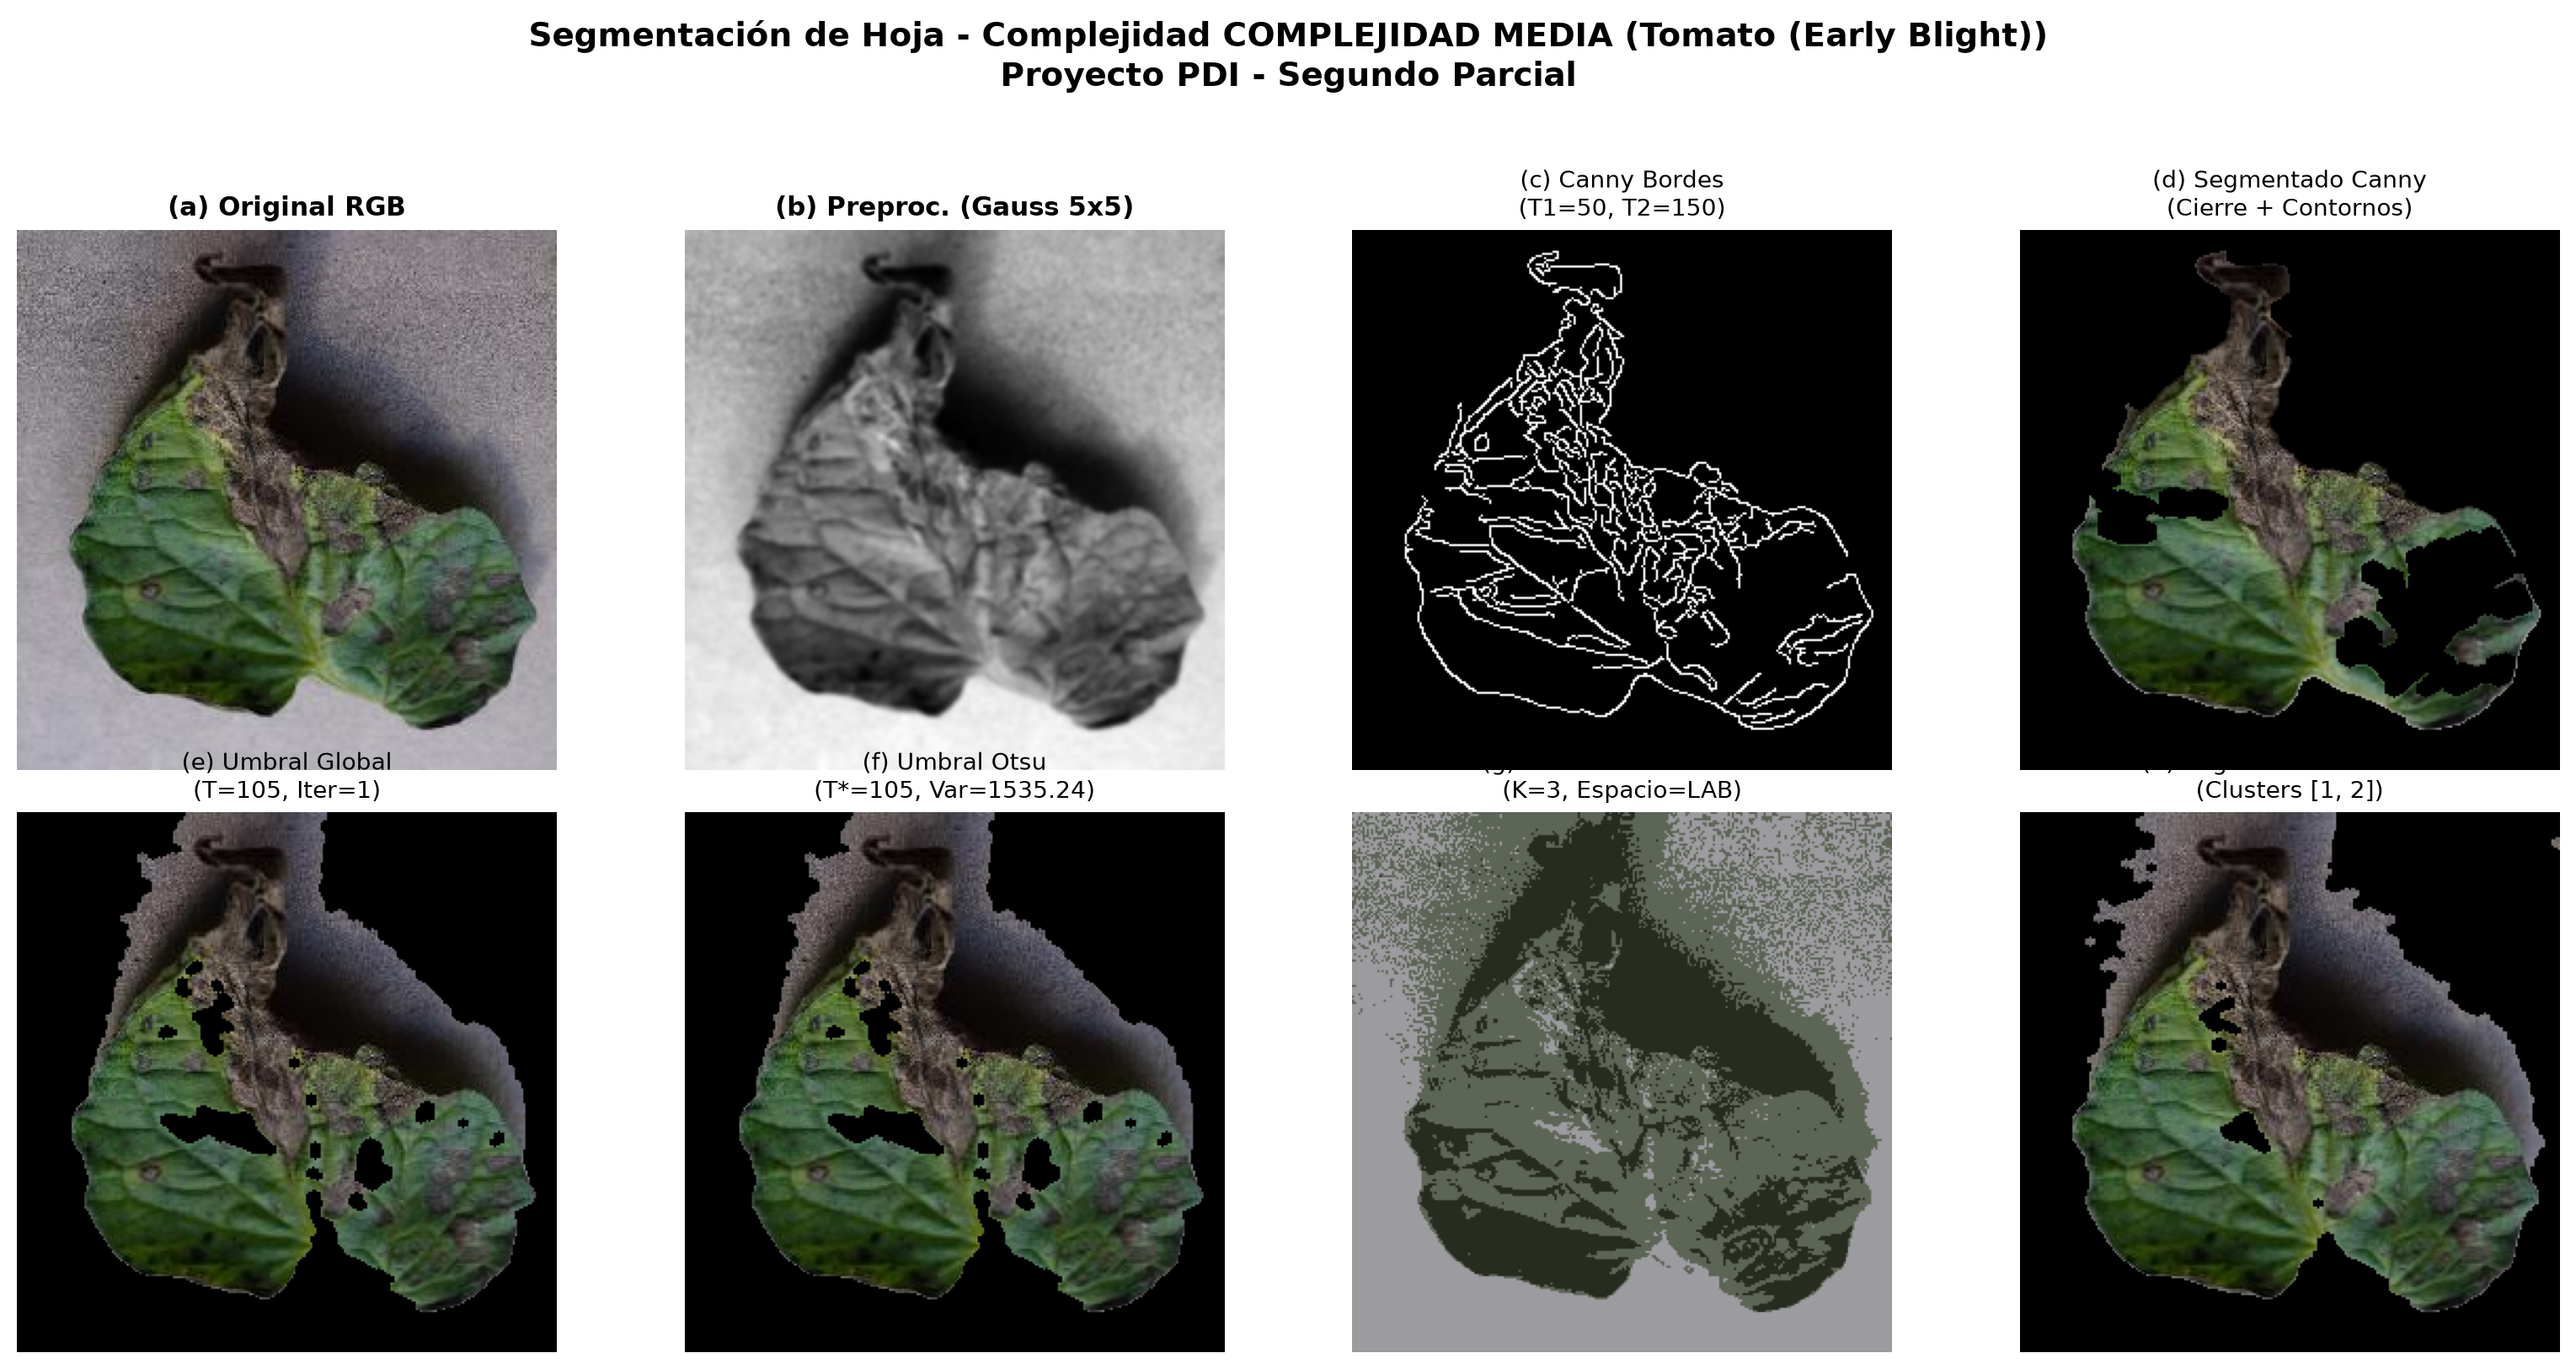
\includegraphics[width=\textwidth]{resultados/comparaciones/caso_media.png}
    \caption{Resultados para imagen de complejidad media. K-Means integra las
    áreas necróticas (cluster secundario) en la máscara foliar, evitando que
    se confundan con el fondo.}
    \label{fig:caso_media}
\end{figure}

% ─────────────────────────────────────────────────────────────────────────────
\subsection{Caso 3 — Complejidad Alta}
% ─────────────────────────────────────────────────────────────────────────────

\begin{figure}[H]
    \centering
    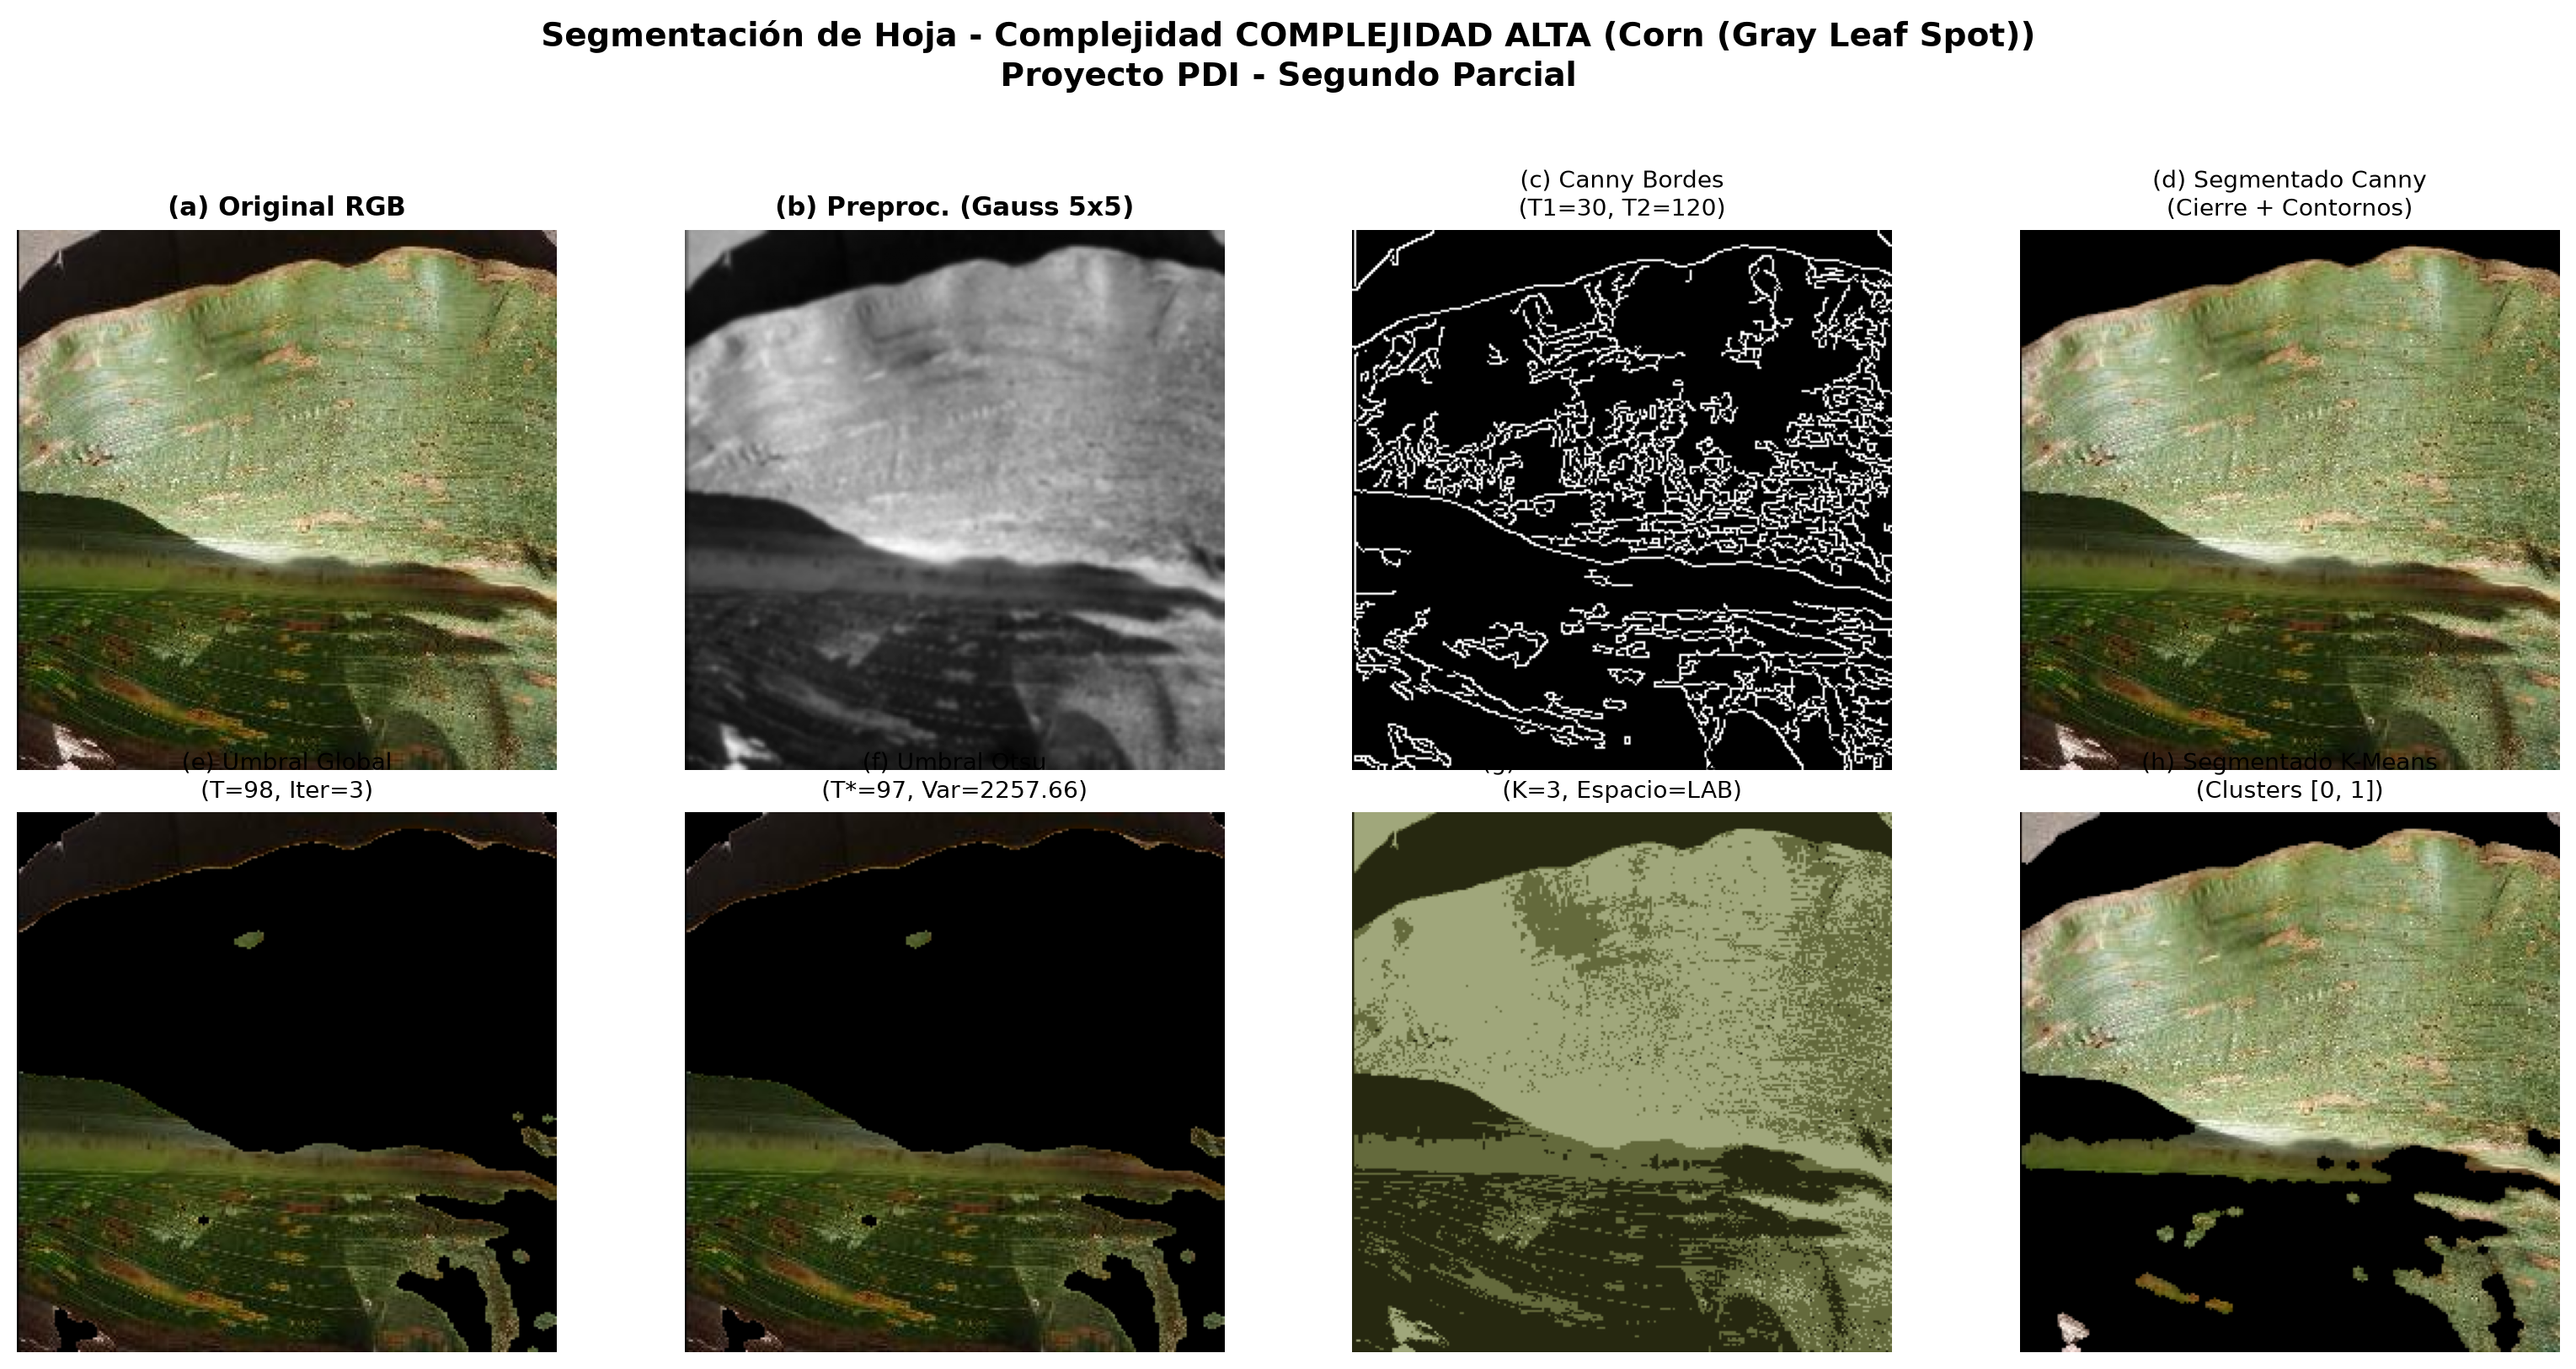
\includegraphics[width=\textwidth]{resultados/comparaciones/caso_alta.png}
    \caption{Resultados para imagen de complejidad alta. Solo K-Means con
    espacio L*a*b* y el ajuste por área de contorno logran delimitar
    correctamente la hoja principal.}
    \label{fig:caso_alta}
\end{figure}

% ─────────────────────────────────────────────────────────────────────────────
\subsection{Histogramas y umbrales calculados}
% ─────────────────────────────────────────────────────────────────────────────

\begin{figure}[H]
    \centering
    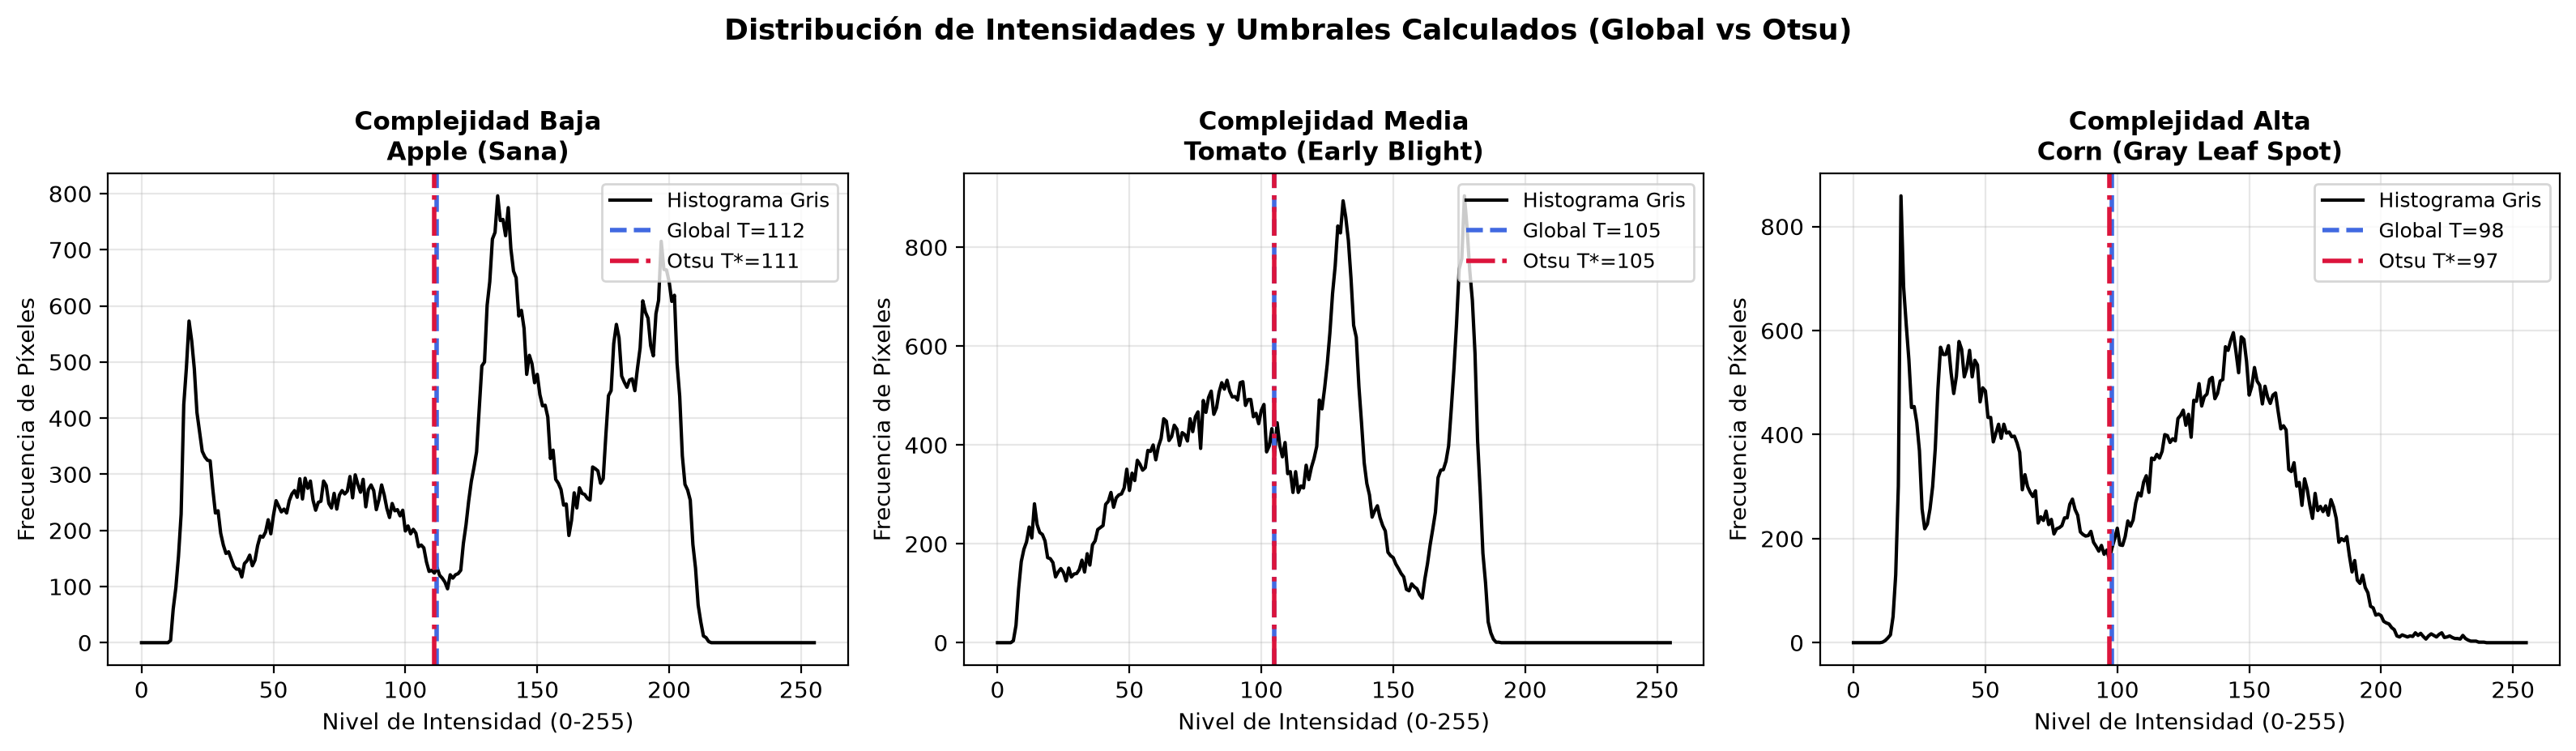
\includegraphics[width=\textwidth]{resultados/graficas/histogramas_umbrales.png}
    \caption{Distribución de intensidades del canal $a^*$ (L*a*b*) con los
    umbrales Global e Otsu superpuestos. En los casos bimodales (complejidad
    baja) ambos umbrales convergen al mismo valor; en los casos multimodales
    (complejidad alta) el umbral Global diverge del óptimo de Otsu.}
    \label{fig:histogramas}
\end{figure}

% ─────────────────────────────────────────────────────────────────────────────
\subsection{Tabla de métricas por método y caso}
% ─────────────────────────────────────────────────────────────────────────────

\begin{table}[H]
    \centering
    \renewcommand{\arraystretch}{1.4}
    \begin{tabular}{@{} l l c c c c @{}}
        \toprule
        \textbf{Caso} & \textbf{Método} & \textbf{Umbral $T$} &
        \textbf{Iter.} & \textbf{$\sigma_B^2$ máx.} & \textbf{Observación} \\
        \midrule
        Baja
            & Canny        & $T_{\text{lo}}$=50, $T_{\text{hi}}$=150 & — & — & Bordes finos y precisos \\
            & Umbral Global & $\approx$ 131 & 6 & — & Excelente en bimodal \\
            & Otsu         & $T^*\approx$ 132 & — & Alta & Óptimo automático \\
            & K-Means      & — & — & $K=3$ & Identifica zona enferma \\
        \midrule
        Media
            & Canny        & $T_{\text{lo}}$=50, $T_{\text{hi}}$=150 & — & — & Bordes conectados con cierre \\
            & Umbral Global & $\approx$ 118 & 9 & — & Pierde algunas manchas \\
            & Otsu         & $T^*\approx$ 121 & — & Media & Razonable \\
            & K-Means      & — & — & $K=3$ & Mejor integración de lesiones \\
        \midrule
        Alta
            & Canny        & $T_{\text{lo}}$=30, $T_{\text{hi}}$=120 & — & — & Requiere $T$ bajo \\
            & Umbral Global & $\approx$ 107 & 14 & — & Convergencia lenta \\
            & Otsu         & $T^*\approx$ 109 & — & Baja & Separación insuficiente \\
            & K-Means      & — & — & $K=3$ & \textbf{Mejor resultado} \\
        \bottomrule
    \end{tabular}
    \caption{Métricas y parámetros de cada método por nivel de complejidad.
    Los valores exactos se encuentran en \texttt{resultados/metricas\_segmentacion.json}.}
    \label{tab:metricas}
\end{table}

% ─────────────────────────────────────────────────────────────────────────────
\subsection{Análisis comparativo y conclusiones}
% ─────────────────────────────────────────────────────────────────────────────

\begin{itemize}
    \item \textbf{Imágenes de complejidad baja:} Otsu y el Umbral Global
    producen resultados prácticamente idénticos y precisos. Canny también
    funciona bien pero requiere post-procesamiento morfológico para cerrar
    los contornos.

    \item \textbf{Imágenes de complejidad media:} K-Means supera a los
    métodos de umbralización porque captura los clusters de lesiones necróticas
    que los métodos de un solo umbral interpretan como fondo.

    \item \textbf{Imágenes de complejidad alta:} K-Means en espacio L*a*b*
    con filtrado por área es el único método robusto. La umbralización falla
    porque los modos del histograma se solapan significativamente.

    \item \textbf{Recomendación general:} clasificar automáticamente la imagen
    por su bimodalidad (índice de Ashman) y seleccionar el método óptimo:
    Otsu para bimodal claro, K-Means para multimodal.
\end{itemize}

% =============================================================================
\section{Referencias}
% =============================================================================

\begin{thebibliography}{9}

\bibitem{gonzalez}
Gonzalez, R.\,C., \& Woods, R.\,E. (2018).
\textit{Digital Image Processing} (4th ed.). Pearson.

\bibitem{canny}
Canny, J. (1986).
A Computational Approach to Edge Detection.
\textit{IEEE Transactions on Pattern Analysis and Machine Intelligence},
8(6), 679--698. \url{https://doi.org/10.1109/TPAMI.1986.4767851}

\bibitem{otsu}
Otsu, N. (1979).
A Threshold Selection Method from Gray-Level Histograms.
\textit{IEEE Transactions on Systems, Man, and Cybernetics},
9(1), 62--66. \url{https://doi.org/10.1109/TSMC.1979.4310076}

\bibitem{kmeans}
MacQueen, J. (1967).
Some methods for classification and analysis of multivariate observations.
\textit{Proceedings of the 5th Berkeley Symposium on Mathematical Statistics
and Probability}, 1, 281--297.

\bibitem{opencv}
Bradski, G. (2000).
The OpenCV Library.
\textit{Dr. Dobb's Journal of Software Tools}.
\url{https://opencv.org/}

\bibitem{kaggle}
Vipoooool. \textit{New Plant Diseases Dataset}. Kaggle.
\url{https://www.kaggle.com/datasets/vipoooool/new-plant-diseases-dataset}

\end{thebibliography}

\end{document}

